\documentclass[a4paper]{report}
\usepackage{float}
\usepackage[utf8]{inputenc}
\usepackage[italian]{babel}
\usepackage{amsmath}
\usepackage{amssymb}
\usepackage{graphicx}
\graphicspath{ {./graph/} }
\usepackage{lmodern}
\usepackage{kpfonts}
\usepackage{titlesec}
\usepackage{listings}
\usepackage{color}
\usepackage{fontspec}
\usepackage{multirow}
\usepackage{float}
\usepackage{array}
\usepackage{dirtree}
\usepackage{afterpage}
\usepackage{enumitem}

\usepackage{fancyvrb}

% Define custom verbatim settings
\DefineVerbatimEnvironment{myverbatim}{Verbatim}{%
  frame=single, % Add a frame around the verbatim text
  framesep=10pt, % Set the separation between the frame and the text
  rulecolor=\color{grigio}, % Set the color of the frame
  fontsize=\small, % Set the font size of the verbatim text
  commandchars=\\\{\} % Allow special characters to be escaped with backslash
}


\setlist[itemize]{label=$\bullet$, leftmargin=0.3cm, itemsep=0.2em}
\usepackage[font={small}, labelfont={bf}, format=hang, skip=8pt]{caption}

\setmonofont{IBM Plex Mono} % Set the monospaced font to IBM Plex Mono
\setmainfont{Helvetica} % Set the main font to Helvetica

% Imposta lo spacing tra il titolo del paragrafo e il testo successivo
\usepackage[left=3.6cm,right=3.6cm,top=2.5cm,bottom=2.25cm]{geometry}

\definecolor{grigio}{rgb}{0.95,0.95,0.95}
\definecolor{mygrey}{rgb}{0.8,0.8,0.8}
\definecolor{mygreen}{rgb}{0.2,0.4,0.2}

\lstset{
    firstnumber=1,                % start line enumeration with line 1000
    numbers=left,
    stepnumber=1,
    numbersep=4pt,
    numberstyle=\tiny\color{mygrey}, % the style that is used for the line-numbers
    backgroundcolor=\color{grigio},
    showspaces=false,
    showstringspaces=false,
    showtabs=false,
    tabsize=3,
    captionpos=b,
    breaklines=true,
    breakatwhitespace=true,
    basicstyle=\ttfamily\fontsize{8pt}{10pt}\selectfont, % Set the basic code style to a smaller font
  keywordstyle=\bfseries\color{blue},  % Stile per i comandi (mov, movb, ...)
  morekeywords={movl, movb, jmp, call},  % Aggiunta dei comandi principali
  commentstyle=\color{mygreen},  % Stile per i commenti
  morecomment=[l]{\#},  % Commenti di una riga che iniziano con #
    moredelim=[il][\color{blue}]{:},  % Etichette
    morekeywords={movl, movb, jmp, call, .byte, jl, addl, addb, decl, dec, jge, jle, cmpb, cmpl, addl,  .int, .ascii, .asciz, .string, jle, je, jz, jg}
}


\titleformat{\chapter}[display]
{\normalfont\huge\bfseries\fontsize{14pt}{10pt}\selectfont}{\chaptertitlename\ \thechapter}{18pt}{\Huge}

\author{Tommi Bimbato VR500751, Antonio Iovine VR504083}
\title{Elaborato Assembly \\ \normalsize Corso di Architettura degli Elaboratori A.A. 2023/2024 \\ Prof.\ Franco Fummi, Prof.\ Michele Lora}

\begin{document}

\begin{titlepage}
  \maketitle
\end{titlepage}

\thispagestyle{empty} % Remove header from title page

\tableofcontents % Add table of contents

\begin{abstract}
  L'obiettivo del progetto è sviluppare un software per la pianificazione delle attività di un sistema produttivo. La produzione è organizzata in slot temporali uniformi, durante i quali un solo prodotto può essere in fase di lavorazione. Il software consentirà di ottimizzare la pianificazione delle attività secondo due algoritmi di pianificazioni differenti. L'intero software è stato sviluppato in linguaggio Assembly (Sintassi AT\&T) e testato su un insieme di dati di prova allegati a questa documentazione.
\end{abstract}

\chapter{Introduzione}
\section{Approccio progettuale}
L'elaborato è stato condotto seguendo un approccio metodologico strutturato. Inizialmente, è stata eseguita un'analisi dettagliata per identificare i requisiti e le funzionalità principali del software. Questo processo ha consentito una comprensione completa del contesto operativo e degli obiettivi da raggiungere.

Successivamente, è stata sviluppata una bozza del software utilizzando il linguaggio di programmazione C. Questo ha permesso la traduzione dei requisiti in una struttura logica e l'identificazione dell'architettura generale del software.

Parallelamente, sono stati definiti gli spazi di memoria necessari per la memorizzazione dei dati durante l'esecuzione del programma. Ciò ha garantito un utilizzo efficiente delle risorse disponibili.

Infine, sono stati eseguiti test approfonditi per verificare il corretto funzionamento del programma e identificare eventuali aree di miglioramento. L'iterazione su questo processo ha portato a modifiche e ottimizzazioni fino al raggiungimento di un livello soddisfacente di prestazioni e funzionalità.

\section{Analisi delle specifiche}
La produzione è organizzata in slot temporali uniformi, durante i quali un solo prodotto può essere in fase di lavorazione. Il programma analizza una serie di prodotti, ognuno caratterizzato da un identificativo, una durata, una scadenza e una priorità secondo le specifiche seguenti:
\begin{itemize}
  \item Identificativo: un codice da 1 a 127;
  \item Durata: il numero di slot temporali per il completamento (da 1 a 10);
  \item Scadenza: il limite massimo di tempo entro cui il prodotto deve essere completato (da 1 a 100);
  \item Priorità: un valore da 1 a 5, che indica sia la priorità che la penalità per il ritardo sulla scadenza\footnote{Il valore 5 indica la priorità più alta.}.
\end{itemize}
Al termine della pianificazione, il programma calcolerà la penale dovuta agli eventuali ritardi di produzione.

\subsection{Input}
L'utente invoca il programma "pianificatore" e fornisce due file come parametri da linea di comando, il primo viene considerato input, mentre il secondo viene utilizzato per salvare i risultati della pianificazione. Ad esempio:q\
\begin{myverbatim}
./Pianificatore Ordini.txt output.txt
\end{myverbatim}
In questo caso, il programma caricherà gli ordini dal file \texttt{Ordini.txt} e salverà le statistiche stampate a video nel file \texttt{output.txt}.
Se l'utente fornisce solo un parametro, il salvataggio della pianificazione su file verrà ignorato.

Il file degli ordini dovrà avere un prodotto per riga, con tutti i parametri separati da virgola. Ad esempio, se l'ordine fosse:
\begin{myverbatim}
ID: 4; Durata: 10; Scadenza: 12; Priorità: 4;
\end{myverbatim}
Il file dovrà contenere la seguente riga:
\begin{myverbatim}
4,10,12,4
\end{myverbatim}

\subsection{Algoritmi di pianificazione}
Una volta letto il file, il programma visualizzerà il menu principale, permettendo all'utente di selezionare l'algoritmo di pianificazione desiderato. Le opzioni disponibili sono:

\begin{enumerate}
  \item Earliest Deadline First (EDF): Si pianificano per primi i prodotti con scadenza più vicina. In caso di parità nella scadenza, si considera la priorità più alta.
  \item Highest Priority First (HPF): Si pianificano per primi i prodotti con la priorità più alta. In caso di parità di priorità, si considera la scadenza più vicina.
\end{enumerate}

L'utente può selezionare uno dei due algoritmi per la pianificazione delle attività del sistema produttivo.

\section{Sviluppo}

\begin{figure}[H]
  \centering
  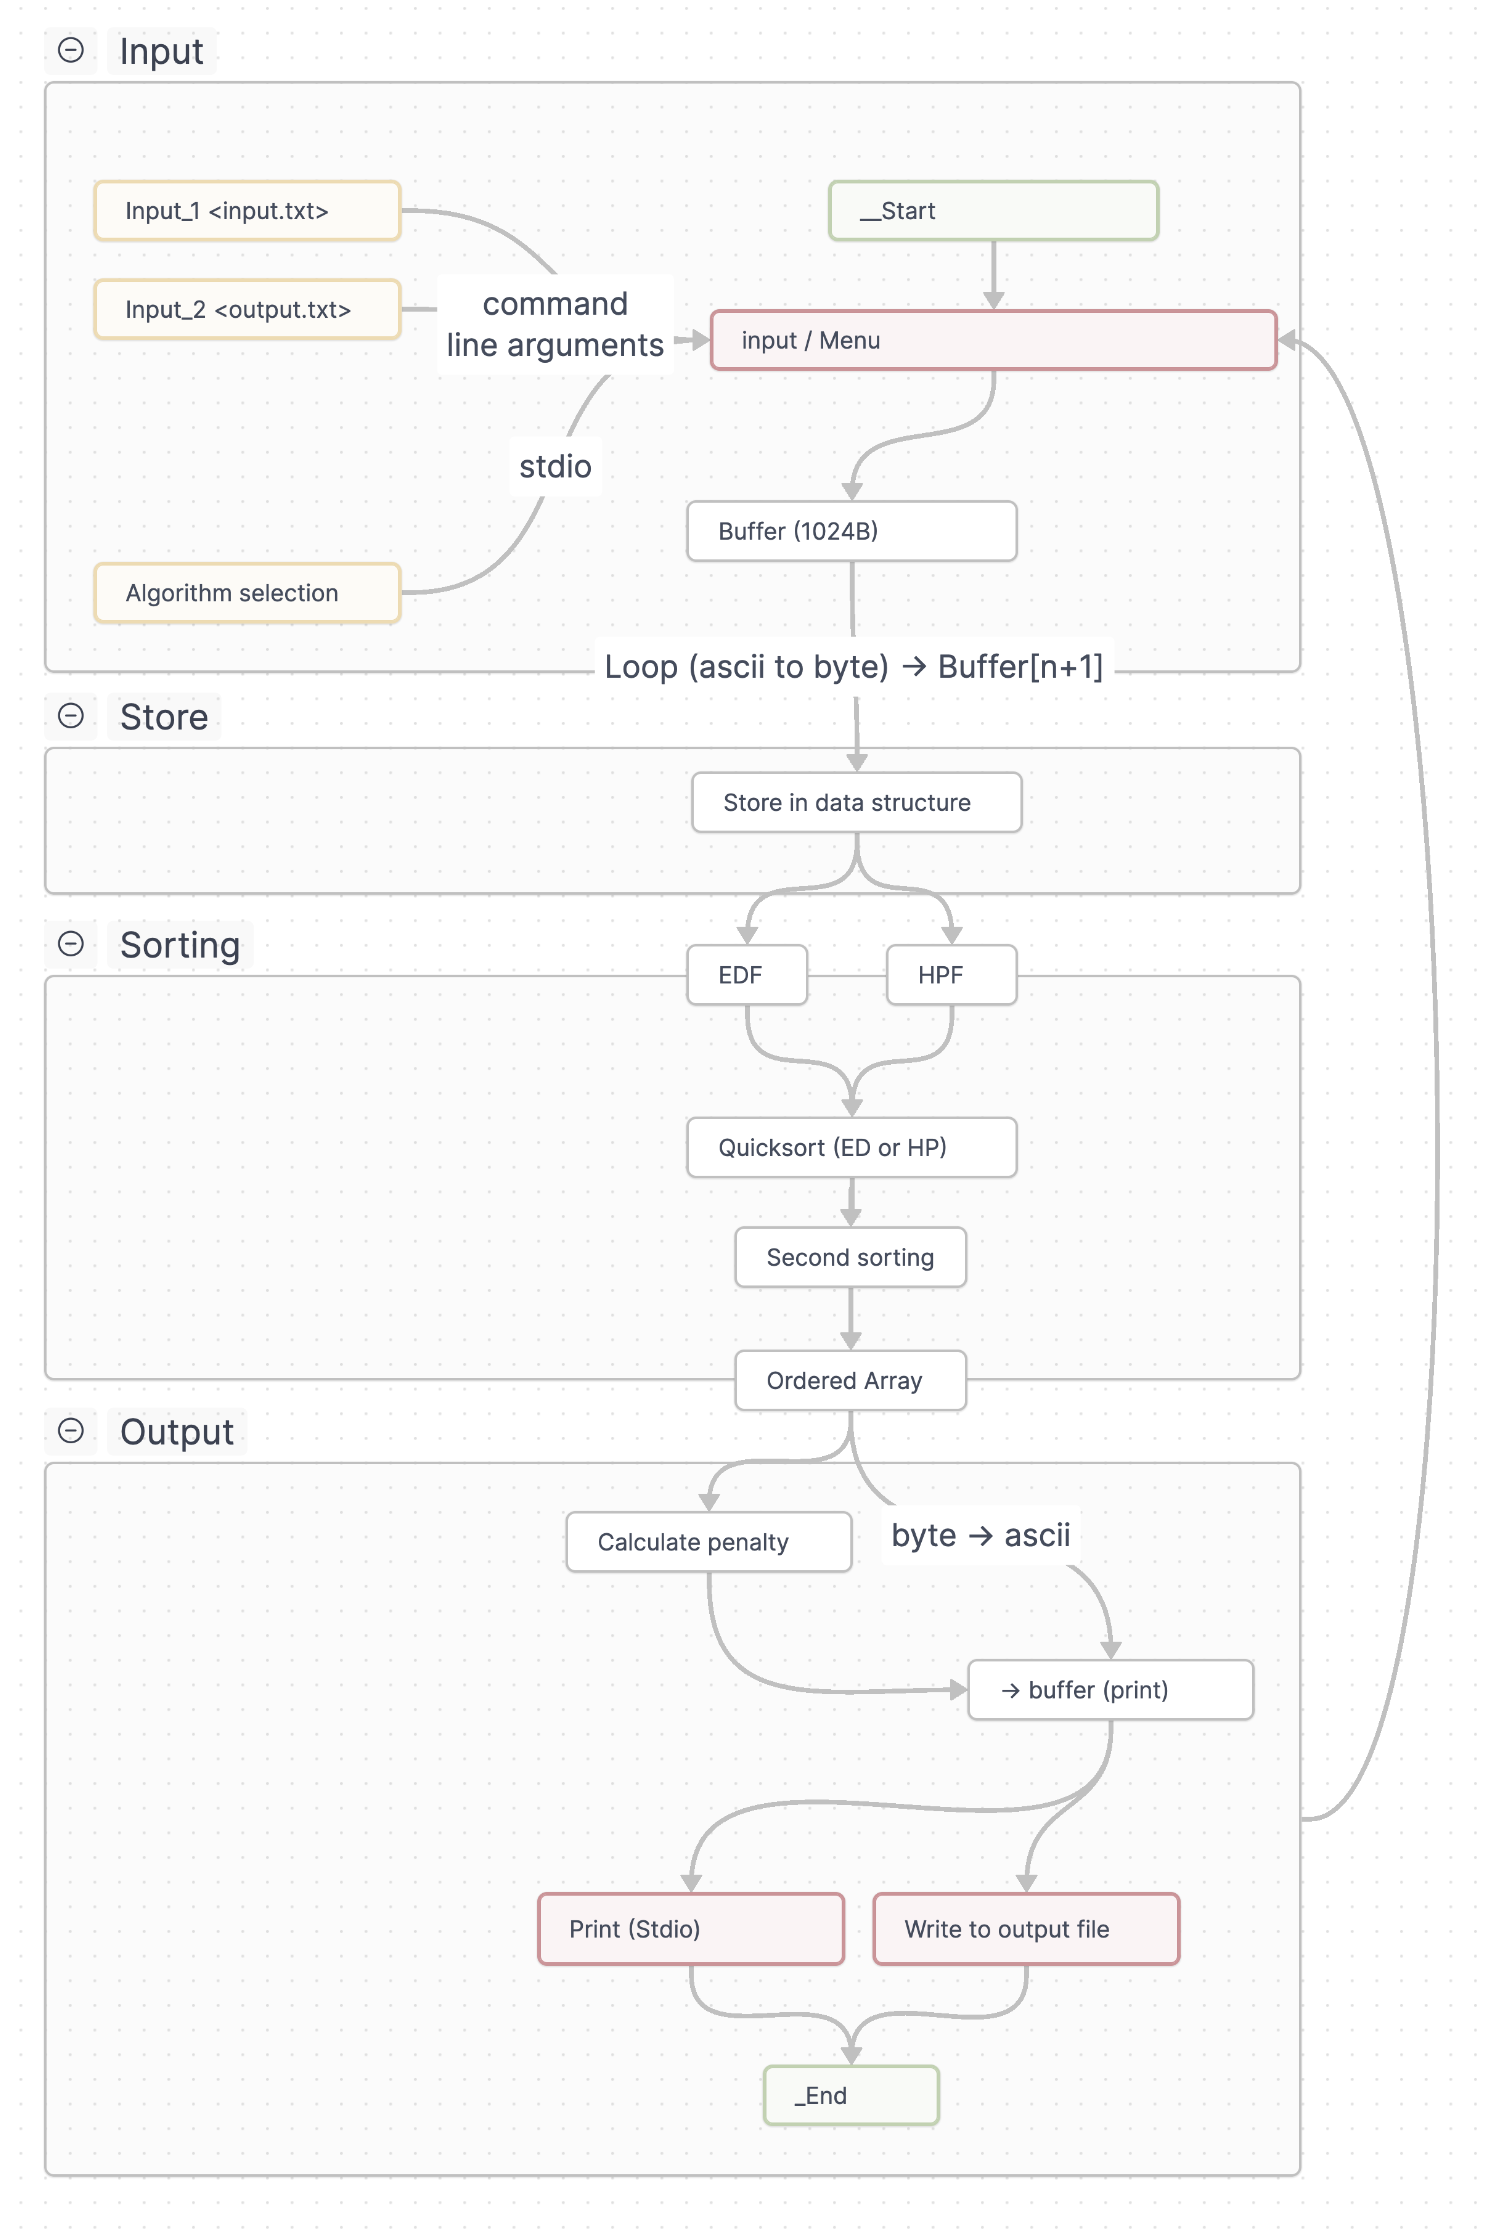
\includegraphics[width=\textwidth]{scheme.png}
  \caption{Schema base del funzionamento del software. [alcune funzionalità sono state omesse per leggibilità dello schema.]}
  \label{fig:schema}
\end{figure}

\subsection{Acquisizione e struttura dati}
Il software acquisisce l'intero contenuto del file di input e lo memorizza in una variabile nel buffer, parallelamente ne calcola la lunghezza (numero di righe) per allocare la memoria necessaria per la struttura dati vera e propria. Successivamente, il programma procede a leggere il contenuto del buffer, converte le informazioni dal formato ASCII al formato numerico e le memorizza in un array di struct. La peculiarità di questa struttura dati è che lo spazio occupato da un prodotto (ID, durata, scadenza e priorità) è di 4 byte totali, pari alla dimensione di un registro interno del processore considerato per l'applicazione del software.

\subsection{Ordinamento dei prodotti}
Acquisita la struttura dati, il programma acquisisce la scelta dell'algoritmo di pianificazione da parte dell'utente e procede con l'ordinamento dei prodotti in base alla scelta effettuata.
Il sorting è gestito da una variabile che definisce la priorità di ordinamento (HPF o EDF) che viene passata alla funzione di ordinamento come parametro. La funzione di ordinamento, a sua volta, si occupa di confrontare i prodotti in base alla priorità scelta e di riordinarli in base a tale criterio nella struttura dati stessa.

Per l'effettivo ordinamento dei prodotti, il software utilizza un algoritmo di sorting di tipo "insertion sort" che si è dimostrato il più efficiente per la dimensione dei dati in ingresso.
Il secondo ordinamento, ovvero quello che compara il parametro "scadenza" in caso di parità di priorità o "priorità in caso di pari scadenza, è gestito da una funzione basata su algoritmo di bubble sort.

\subsection{Output}
Nel caso venisse specificato un file di output, il software stamperà su di esso i risultati della pianificazione secondo il seguente schema:


\begin{myverbatim}
<Algoritmo di pianificazione scelto>:
<ID del prodotto>:<Inizio produzione>
[...]
Conclusione:<timeslot termine produzione>
Penalty:<penalità totale>
\end{myverbatim}


\small{Esempio:}

\begin{myverbatim}
Pianificazione EDF:
1:0
4:2
\dots
9:55
Conclusione: 63
Penalty: 0
  \end{myverbatim}
L'output della pianificazione viene comunque visualizzato a video.

\subsection{Penalità}
Se un prodotto non viene completato entro la scadenza, il programma calcola la penalità in base alla priorità del prodotto e alla quantità di slot temporali di ritardo. La penalità è calcolata come segue:

\[
\text{Penalità} = \text{Priorità} \times \text{Ritardo}
\]

\newpage
\section{Codice}

\subsection{Struttra della cartella di progetto}

\dirtree{%
.1 VR500751\_VR504083.
.2 bin.
  .3 *Pianificatore*.
.2 obj.
.2 Ordini.
  .3 EDF.txt.
  .3 NONE.txt.
  .3 BOTH.txt.
.2 src.
  .3 AskInput.s.
  .3 AskOutput.s.
  .3 btoa.s.
  .3 BufferToArray.s.
  .3 EqualSort.s.
  .3 FinalData.s.
  .3 InsertionSort.s.
  .3 Intestazione.s.
  .3 menu.s.
  .3 main.s.
  .3 textin.s.
.2 Makefile.
}

\subsection{File sorgenti}

\subsubsection{Il programma è composto dai seguenti file sorgente in linguaggio assembly:}
\begin{itemize}
  \item \texttt{AskInput.s}: funzione per richiedere il nome del file di input all'utente;
  \item \texttt{AskOutput.s}: funzione per richiedere il nome del file di output all'utente;
  \item \texttt{textin.s}: funzione per la lettura di una scelta da tastiera.
  \item \texttt{btoa.s}: funzione loop per la conversione di un byte in ASCII;
  \item \texttt{BufferToArray.s}: funzione per la conversione del buffer di lettura in un array di struct;
  \item \texttt{EqualSort.s}: funzione per il secondo ordinamento dei prodotti;
  \item \texttt{FinalData.s}: funzione per la stampa dei risultati della pianificazione;
  \item \texttt{InsertionSort.s}: funzione per il primo ordinamento dei prodotti;
  \item \texttt{Intestazione.s}: scrittura dell'intestazione condizionale dell'output del programma;
  \item \texttt{menu.s}: file contenente la funzione per l'invocazione del menù utente;
  \item \texttt{main.s}: funzione principale del programma;
\end{itemize}
\

\subsubsection{Alcuni stralci di codice significativi:}

  \begin{itemize}
    \item Allocazione della memoria \texttt{main.s}:
    \begin{lstlisting}[firstnumber=130]
    malloc:                 # alloca spazio per l'array

    movl len, %eax
    sal $2, %eax            # moltiplico per 4 (4byte per int) (perchè ho 4byte ogni riga/prodotto)     
    movl %eax, len

    movl $45, %eax          # syscall per la malloc
    xorl %ebx, %ebx         # alloco inizialmente 0byte
    int $0x80   
    
    movl %eax, %esi         # salvo l'indirizzo di memoria in esi (zona di memoria puntata dalla malloc)
    
    addl len, %eax          # aggiungo len a %eax (buffer allocazione)
                                                              
    movl %eax, %ebx         # salvo il risultato in ebx (lunghezza totale da allocare)
    movl $45, %eax          # syscall per la malloc
    int $0x80               # alloco la memoria - interrupt
    
    cmpl %esi, %eax         # compara nuovo puntatore col vecchio (se sono uguali non ha allocato)
    jle Error               # esi è l'indirizzo di memoria puntato dalla malloc (inizio array) mentre in eax c'è l'indirizzo di fine array
    
    movl %esi, ArrayPointer # se tutto funziona salvo l'indirizzo di memoria in ArrayPointer cosi lo posso usare in BufferToArray
    
    \end{lstlisting}
    
    \item Insertion sort \texttt{insertionSort.s}:
    \begin{lstlisting}[firstnumber=1]
  .section .data

    key: .int 0
    base: .int 0

.section .text 
    .global insertionSort
    .type insertionSort, @function

insertionSort:

    pushl %ebp
    movl %esp, %ebp

    movl 8(%ebp), %edi # edi = Arr[fine]
    movl 12(%ebp), %esi # esi = Arr[inizio]
    movl 16(%ebp), %ecx # Metodo di sorting (+3 Priorità, +2 Scadenza)

    popl %ebp

    movl %ecx, base

    xorl %ecx, %ecx # i = 0
    xorl %edx, %edx # j = 0
    addl base, %ecx # %ecx punta alla priorità/scadenza 
    addl $4, %ecx  # %punta a 2 oggetto (1)

for:

    cmpl %ecx, %edi
    jle endFor

    movl (%esi, %ecx, 1), %eax
    movb %al, key 
    subl base, %ecx
    movl (%esi, %ecx, 1), %eax
    push %eax
    addl base, %ecx

    movl %ecx, %edx # j = i
    addl $-4, %edx # j = i - 1

while:

    cmpl $0, %edx
    jl PrepEndWhile

    movb (%esi,%edx,1), %al

    cmpb %al, key
    jg PrepEndWhile

    subl base, %edx
    movl %edx, %eax
    addl $4, %eax
    movl (%esi ,%edx,1), %ebx
    movl %ebx, (%esi ,%eax,1)
    decl %edx

    cmpl $3, base
    je while

    decl %edx

    jmp while

PrepEndWhile:

    incl %edx

    cmpl $3, base
    je endWhile

    incl %edx

endWhile:

    popl %eax
    movl %eax, (%esi ,%edx, 1)

    addl $4, %ecx

    jmp for

endFor:

    ret
    \end{lstlisting}
    
    \item Bubble sort \texttt{equalSort.s}:
    
    \begin{lstlisting}[firstnumber=1]
.section .data

base: .byte 0               # EDF or HPF
flag: .byte 0               # 1 -> swap 0 -> no swap

.section .text
    .global EqualSort
    .type EqualSort, @function

EqualSort:

    pushl %ebp              
    movl %esp, %ebp
 
    movl 8(%ebp), %edi      #len
    movl 12(%ebp), %esi     #pointer
    movl 16(%ebp), %ecx     #Base

    popl %ebp               #restore stack

    movb %cl, base          #salvo base (EDF or HPF)
    movl %ecx, %eax         # i
    movl %eax, %ebx         # j
    addl $4, %ebx           # j + 1

loop:

    cmpl %eax, %edi         #len <= i (uscita)
    jle endLoop

    xorl %ecx, %ecx
    xorl %edx, %edx

    movb (%esi, %eax, 1), %cl   
    movb (%esi, %ebx, 1), %dl

    cmpb %cl, %dl               #confronto i e j
    je Check                    #se sono uguali vado a check

    jmp next

Check:

    cmpb $3, base               #se base = HPF (priorità) -> decrement
    je decrement

increment:                      # guardo priorità

    incl %eax                   #incremento i
    incl %ebx                   #incremento j

    movb (%esi, %eax, 1), %cl       # preparo il confronto dei prossimi valori
    movb (%esi, %ebx, 1), %dl


    subl $3, %eax           # torno a puntare l'inizio dell'elemento
    subl $3, %ebx           # =

    cmpb %cl, %dl           # confronto i e j
    jl reset                
    je SetDurata

    movl (%esi, %eax, 1), %ecx
    movl (%esi, %ebx, 1), %edx

    movl %ecx, (%esi, %ebx, 1)
    movl %edx, (%esi, %eax, 1)

    movb $1, flag

    jmp reset

decrement:                  # guardo scadenza

    decl %eax
    decl %ebx

    movb (%esi, %eax, 1), %cl
    movb (%esi, %ebx, 1), %dl


    subl $2, %eax
    subl $2, %ebx

    cmpb %dl, %cl
    jg reset
    je SetDurata

    movl (%esi, %eax, 1), %ecx
    movl (%esi, %ebx, 1), %edx

    movl %ecx, (%esi, %ebx, 1)
    movl %edx, (%esi, %eax, 1)

    movb $1, flag

    jmp reset

SetDurata:        # se scadenza uguale priorità uguali, controllo la durata

    addl $1, %eax    # incremento così vado da ID a durata
    addl $1, %ebx

Durata:

    movb (%esi, %eax, 1), %cl
    movb (%esi, %ebx, 1), %dl


    subl $1, %eax
    subl $1, %ebx

    cmpb %cl, %dl
    jge reset
    
    movl (%esi, %eax, 1), %ecx
    movl (%esi, %ebx, 1), %edx

    movl %ecx, (%esi, %ebx, 1)
    movl %edx, (%esi, %eax, 1)

    movb $1, flag

reset:

    addb base, %al     # resetto base
    addb base, %bl     # resetto base

next:

    cmpb $1, flag
    je Redo

    addl $4, %eax
    addl $4, %ebx
    jmp loop

Redo:                   # se ho fatto uno swap, ripeto il confronto

    movl $0, flag
    movl base, %ecx
    movl %ecx, %eax
    movl %eax, %ebx
    addl $4, %ebx

    jmp loop

endLoop:
    
    ret
    
    \end{lstlisting}


    
    \item Loop scrittura \texttt{FinalData.s}:
    
    \begin{lstlisting}[firstnumber=1]
.section .data

PenaltyMsgLen: .byte 9
TimeMsgLen: .byte 13

PenaltyMsg: .string "Penalty: "
TimeMsg: .string "Conclusione: "

timeAscii: .byte 4
penaltyAscii: .byte 6


.section .text
    .globl finalData
    .type finalData, @function

finalData:

    pushl %ebx #salvo la penalita'
    pushl %eax #salvo il tempo
    addl %edx, %edi # aggiungo la lunghezza del buffer all'inizio del buffer per avere il primo spazio libero
    xorl %ecx, %ecx #per sicurezza azzero ecx

    movl $TimeMsg, %esi
    movb TimeMsgLen, %cl
    cld                      # flag reset direction
    LoopTime:                # ctrl c e ctrl v
        lodsb                # carica byte da %esi ad %al
        stosb                # scrive byte da %al a %edi
        loop LoopTime        # decrementa %cl e se non è zero salta a LoopTime


getTime:        # Tempo in numeri in %ebx e dove scrivere in %edi

    popl %eax   # Riprendo dalla stack il tempo
    movl $10, %ebx     
    leal timeAscii+3, %esi    #un semplicissimo btoa che trasforma il tempo in ascii 
    movl $10, (%esi)

loopTime_B:

    xorl %edx, %edx         # pulisco edx
    divl %ebx               # divido per prendere il resto

    addb $48, %dl           #aggiungo 48 per trasformare il numero in ascii
    decl %esi               #decremento il puntatore che fino a questo punto punta a 10 (vedi sopra)
    movb %dl, (%esi)       

    test %eax, %eax       
    jz BufferTime

    jmp loopTime_B

BufferTime: # copio il buffer in %edi(puntatore al buffer)

    movb (%esi), %al
    cmpb $10, %al
    je next
    movb %al, (%edi)

    incl %edi   
    incl %esi

    jmp BufferTime

next:  #finito il tempo uso il tappo \n

    movb $10, (%edi)
    incl %edi

    xorl %ecx, %ecx 

    movl $PenaltyMsg, %esi
    movb PenaltyMsgLen, %cl
    cld                                # ctrl c e ctrl v
    LoopPenalty:
        lodsb
        stosb
        loop LoopPenalty

getPenalty: 

    popl %eax # Riprendo dalla stack la penalita'
    movl $10, %ebx     
    leal penaltyAscii+5, %esi 
    movl $10, (%esi)

loopPenalty:

    xorl %edx, %edx
    divl %ebx

    addb $48, %dl
    decl %esi
    movb %dl, (%esi)    # 'time loop' ma per la penalita'

    test %eax, %eax     # se è 0 esco
    jz BufferPenalty    # altrimenti continuo

    jmp loopPenalty

BufferPenalty:

    movb (%esi), %al
    cmpb $10, %al
    je end
    movb %al, (%edi)

    incl %edi
    incl %esi

    jmp BufferPenalty

end:

    movb %al, (%edi)      #aggiungo \n
    
    ret

    \end{lstlisting}
    

  \end{itemize}

\subsubsection{In allegato si troveranno i seguenti dataset per testare il programma:}
\begin{itemize}
  \item \texttt{Makefile}: file per la compilazione del programma;
  \item \texttt{EDF.txt}: file di input con penalità uguale a zero con EDF e maggiore di zero con HPF;
  \item \texttt{BOTH.txt}: file di input con penalità uguale a zero con entrambi gli algoritmi;
  \item \texttt{NONE.txt}: file di input con penalità maggiore di zero con entrambi gli algoritmi.
\end{itemize}

\section{Scelte progettuali}

  \subsection{Ouput su file / funzioni extra-specifiche}
  Durante la programmazione del software sono state implementate alcune funzionalità aggiuntive:
    \begin{itemize}
      \item Salvataggio dei risultati della pianificazione su file;
      \item Visualizzazione del menù utente multi-scelta;
      \item Possibilità di lanciare il software senza specificare un file di output.
      \item Modifica a runtime di file di input e output.
      \item Visualizzazione di un messaggio di errore nel caso di file di output non non specificato.
    \end{itemize}

  \subsection{Algoritmi di sorting}
  Per l'ordinamento dei prodotti, sono stati implementati due algoritmi di sorting differenti:

    \begin{itemize}
      \item \texttt{Sorting principale}: ordinamento basato su algoritmo 'insertion sort' per il confronto diretto tra il valore indicato dalla tipologia di pianificazione (EDF: deadline, HPF: priorità);
      \item \texttt{Sorting secondario}: ordinamento secondario basato su algoritmo di tipo 'bubble sort' per il confronto in caso di valore principale identico.
    \end{itemize}
    
    \subsection{Limiti del software}
    Durante la fase di testing sono sorte alcune limitazioni del software:

      \begin{itemize}
        \item Il software non è in grado di gestire generalmete prodotti con valori maggiori di 256;
        \item Il software non è in grado di gestire file di input aventi dimensione maggiore di 1024 Byte.
        \item Il software non è in grado di gestire file di output aventi dimensione maggiore di 1024 Byte.
      \end{itemize}



\end{document}